% This file was created by tikzplotlib v0.9.8.
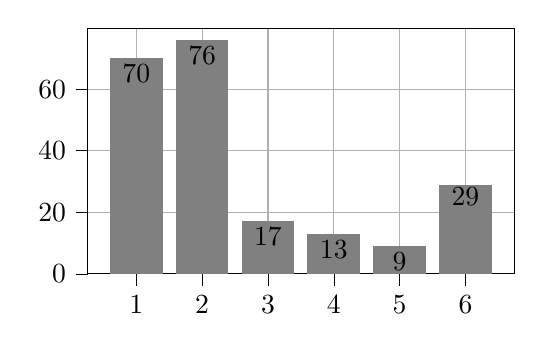
\begin{tikzpicture}\footnote{\textcolor{red}{check classes for this dataset. One class is missing.}}

\begin{axis}[
tick align=outside,
tick pos=left,
%title={Distribution between classes for glass dataset},
x grid style={white!69.0196078431373!black},
xmajorgrids,
xmin=0.26, xmax=6.74,
xtick style={color=black},
xtick={1,2,3,4,5,6},
xticklabels={1,2,3,4,5,6},
y grid style={white!69.0196078431373!black},
ymajorgrids,
ymin=0, ymax=79.8,
ytick style={color=black},
height=4.7cm,
width=7cm,
]
\draw[draw=none,fill=white!50.1960784313725!black] (axis cs:0.6,0) rectangle (axis cs:1.4,70);
\draw[draw=none,fill=white!50.1960784313725!black] (axis cs:1.6,0) rectangle (axis cs:2.4,76);
\draw[draw=none,fill=white!50.1960784313725!black] (axis cs:2.6,0) rectangle (axis cs:3.4,17);
\draw[draw=none,fill=white!50.1960784313725!black] (axis cs:3.6,0) rectangle (axis cs:4.4,13);
\draw[draw=none,fill=white!50.1960784313725!black] (axis cs:4.6,0) rectangle (axis cs:5.4,9);
\draw[draw=none,fill=white!50.1960784313725!black] (axis cs:5.6,0) rectangle (axis cs:6.4,29);

\node[draw=none,align=center] at (axis cs:1,65) {70};
\node[draw=none,align=center] at (axis cs:2,71) {76};
\node[draw=none,align=center] at (axis cs:3,12) {17};
\node[draw=none,align=center] at (axis cs:4,8) {13};
\node[draw=none,align=center] at (axis cs:5,4) {9};
\node[draw=none,align=center] at (axis cs:6,25) {29};

\end{axis}


\end{tikzpicture}
